\subsection{Czujnik światła}
\label{sec:czujnik_swiatla}
Inteligentna donica wykorzystuje czujnik światła oparty na protokole komunikacyjnym I2C. Implementacja tego elementu obejmuje trzy kluczowe funkcjonalności:
ISL29003 to zintegrowany czujnik światła z 16-bitowym przetwornikiem ADC. Wewnętrzny przetwornik ADC zapewnia 16-bitową rozdzielczość. Ogólne zasady działania ADC zostały przedstawione w rozdziale \ref{sec:ADC}.

\begin{enumerate}
    \item \textbf{Inicjalizacja i konfiguracja czujnika ISL29003} - Proces inicjalizacji obejmuje ustawienie adresu urządzenia na magistrali I2C, konfigurację rejestrów czujnika oraz określenie parametrów pomiaru, takich jak czułość i częstotliwość próbkowania.

    \item \textbf{Odczyt danych z czujnika} - Funkcjonalność ta odpowiada za komunikację z czujnikiem poprzez protokół I2C, wysyłanie komend odczytu do odpowiednich rejestrów oraz interpretację otrzymanych danych. Implementacja uwzględnia obsługę błędów komunikacji oraz weryfikację poprawności odczytanych wartości.

    \item \textbf{Przetwarzanie i analiza danych} - Po odczytaniu surowych danych z czujnika, system przetwarza je na użyteczne informacje o poziomie natężenia światła. Funkcjonalność ta obejmuje kalibrację, filtrowanie zakłóceń oraz konwersję wartości na jednostki zrozumiałe dla użytkownika (np. luxy).
\end{enumerate}

\subsubsection{Inicjalizacja czujnika ISL29003}
    Aby zainicjować czujnik ISL29003, należy ustawić wartość 1 na 7. bicie rejestru Command (0x00). Sposób wysyłania zawartości rejestrów do urządzeń podrzędnych zostałopisany w poprzednim podrozdziale \hyperref[I2C_wysylanie_rejestrow]{o I2C}.% \ref{sec:I2C_wysylanie_rejestrow}.

    Wysyłanie adresu urządzenia ISL29003 na magistrali I2C - adres urządzenia to 0x44.\\
    Informacje na temat rejestrów i ich wartości znajdują się w \href{https://www.zsk.p.lodz.pl/~morawski/SCR&ES/NotyKatalogowe/ISL29003.pdf}{dokumentacji ISL29003 (Tabela 1)}.\\

    Kolejnym etapem przygotowania czujnika do pracy jest zdefiniowanie zakresu. Stałe te będą używane do przeliczania danych wyjściowych czujnika. W naszym programie ustawiamy zakres na 3892, co oznacza skalę od 0 do 3892 lux. Aby ustawić wybrane przez nas wartości zakresu (range) należy sutawić bity 3:2 (tabela 9.) w rejestrze Control (0x01) na 0:1
%tabela 9.
    \begin{table}[H]
        \centering
        \begin{tabular}{|c|c|c|}
        \hline
        \rowcolor{gray!30}
        Bits 3:2 & k & RANGE (k)\\
        \hline
        0:0 & 1 & 973\\
        \hline
        0:1 & 2 & 3892\\
        \hline
        1:0 & 3 & 15,568\\
        \hline
        1:1 & 4 & 62,272\\
        \hline
        \end{tabular}
        \caption{Zakresy skali lux}
    \end{table}
    Ustawiamy także liczbę cykli zegara na konwersację analogowo cyfrową poprzez umieszczenie wartości 0:0 na bitach 1:0 w rejestrze Command (0x00) (tabela 7.)
    \begin{table}[H]
        \centering
        \begin{tabular}{|c|c|}
        \hline
        \rowcolor{gray!30}
        BITS 1:0 & NUMBER OF CLOCK CYCLES\\
        \hline
        0:0 & $2^{16} = 65,536$\\
        \hline
        0:1 & $2^{12} = 4,096$\\
        \hline
        1:0 & $2^{8} = 256$\\
        \hline
        1:1 & $2^{4} = 16$\\
        \hline
        \end{tabular}
        \caption{Liczby cykli zegara}
    \end{table}

    \subsubsection{Odczyt danych z czujnika}
    Dane z ISL29003 odczytujemy przy pomocy protokołu I2C. Dane wyjściowe przechowywane są w dchów rejestrach, ponieważ odczyt jest liczbą 16-bitową. W rejestrze o adresie 0x04 znajduje się najniższy bajt danych, a w rejestrze 0x05 najwyższy bajt. Sposób odczytywania danych został opisany w podrozdziale \ref{sec:I2C_wysylanie_rejestrow}.

    \subsubsection{Przetwarzanie i analiza danych}
    Po odczytaniu danych z czujnika, system przetwarza je na użyteczne informacje o poziomie natężenia światła. Aby uzyskać wartość w luxach, należy zastosować poniższy wzór (ten wzór obowiązuje tylko gdy mamy zewnętrzny rezystor 100k$\Omega$):
    \begin{equation}
        E = \frac{FSR \cdot DATA}{2^{n}}
    \end{equation}

    Gdzie:
    
    \quad E - wartość w luxach 

    \quad FSR - zakres skali (FSR = 3892 lux) 

    \quad DATA - odczytana wartość z rejestru

    \quad n - liczba bitów w rejestrze (16 bitów)
   


    %wstawienie zdjęcia
    \begin{figure}[H]
        \centering
        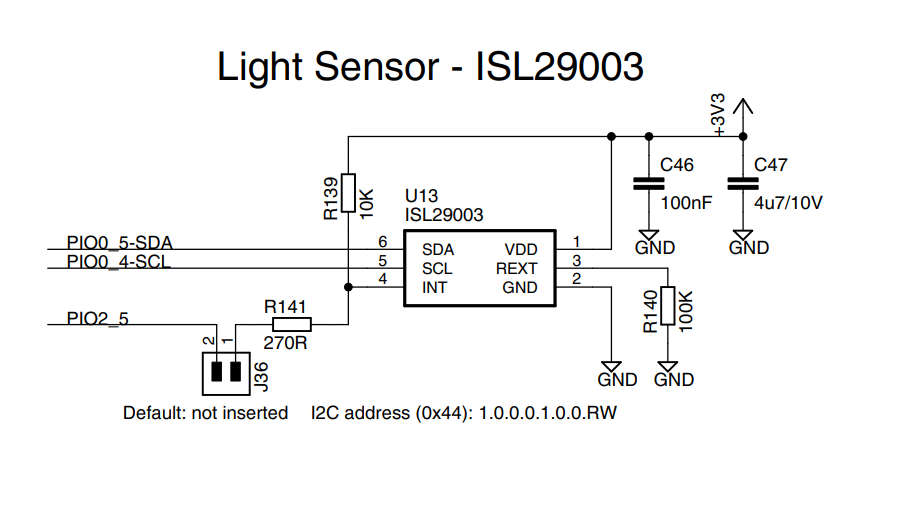
\includegraphics[width=0.8\textwidth]{../ISL29003/schemat.png}
        \caption{Schemat podłączenia czujnika ISL29003}
        \label{fig:czujnik_swiatla}
    \end{figure}
